% Préambule APMEP - Annales
% Auteurs
% tapuscrit : François Kriegk
% relecture :
% figures TikZ : François Kriegk
% figures pstricks : François Hache
% modifications :
% Remerciements :
% version 2 : 2026-07-01
%
\documentclass[12pt,a4paper,french]{article}

% Packages
%%% codage et police utilisée
\usepackage[T1]{fontenc}
\RequirePackage{iftex}
\iftutex % moteur utf-8 lualatex, xelatex
	\usepackage{fourier-otf} % remplace fourier pour moteur utf8 (LuaLaTeX, XeLaTeX)
	% Alternatives nécéssite (LuaLaTeX, XeLaTeX)
    \usepackage{hyperref}
	%\usepackage{fontspec}% pour utiliser des fontes système
\else % pour les autres moteurs latex, pdflatex
	\usepackage[utf8]{inputenc}
	\usepackage{fourier}
	\usepackage{amsmath,amssymb}
    \usepackage[dvips]{hyperref}
    \renewcommand{\ttdefault}{lmtt}
\fi
\usepackage[normalem]{ulem}
\usepackage{pifont}
\usepackage{lscape}
% tableaux
\usepackage{multicol}
\usepackage{multirow}
\usepackage{tabularx}
\usepackage{tabularray}
% texte et composition
\usepackage{textcomp}
\usepackage{babel}
\usepackage[np]{numprint}
%
\usepackage{fancyhdr}
\usepackage{makeidx}
\makeindex
% pour le symbole €
\usepackage{eurosym}
\DeclareRobustCommand{\officialeuro}{%
  \ifmmode\expandafter\text\fi
  {\fontencoding{U}\fontfamily{eurosym}\selectfont e}}
\AtBeginDocument{\renewcommand{\euro}{\officialeuro}}
% couleurs étendues
\usepackage{xcolor}
% pour les listes
\usepackage{enumitem}
% Enumérations réglage par défaut
\setlist[itemize]{label=\textbullet,leftmargin=5mm,labelwidth=3mm,labelsep=2mm,align=left}
\setlist[enumerate]{labelindent=0pt, leftmargin=5mm, labelsep=2mm, labelwidth=3mm,labelsep=2mm, align= left}
\setlist[enumerate,1]{label = \textbf{\arabic*.}}
\setlist[enumerate,2]{label = \textbf{\alph*.}}
\setlist[enumerate,3]{label = \textbf{\roman*.}}
% pour l'ajustement des boites (figures…)
\usepackage{adjustbox}
% pour ne pas commencer un exercice en fin de page
\usepackage{needspace}
%
% Taille de la zone d'écriture
\usepackage[left=1.5cm,right=1.5cm,top=3cm,bottom=3cm]{geometry}
\setlength{\headheight}{15pt}
\setlength{\parindent}{0mm}
%
% Formatage du pdf
\hypersetup{%
    pdfauthor = {APMEP},
    pdfsubject = {Troisième, générale},
    pdftitle = {Brevet des collèges -- Session 2026 -- },
    allbordercolors = white,
    pdfstartview=FitH
}
% Pour scratch (code)
\usepackage{scratch3}
% Pour le code Python
\usepackage{listings}
\lstdefinestyle{python}{
  language=Python,
  basicstyle=\ttfamily\small,
  keywordstyle=\color{blue}\bfseries,
  commentstyle=\color{gray}\itshape,
  stringstyle=\color{orange},
  numbers=left,
  numberstyle=\tiny\color{gray},
  breaklines=true,
  frame=single,
  backgroundcolor=\color{gray!5},
  tabsize=4
}
  % usage (exemple)
  %\begin{lstlisting}[style=python]
%def seuil():
%    n = 1
%    p = 0.5
%    while p < 0.6 :
%       n = n + 1
%       p = p*7/15 + 1/3
%    return n
%\end{lstlisting}


% Pour une visualisation de type tableur
\usepackage{pas-tableur}
%
%% pour PsTricks
\usepackage{pst-bezier}%% AVANT les autres PST
\usepackage{pstricks-add}
\usepackage{pst-func,pst-tree,pst-circ}
\usepackage{pst-eucl}
%% pour TikZ
\usepackage{tikz,pgfplots,pgf,tkz-tab,tikzpagenodes}
\usetikzlibrary{calc,patterns,decorations,arrows.meta,patterns.meta,arrows}
\pgfplotsset{compat=1.18,/pgf/number format/.cd,use comma}
\usepackage{icomma} % gestion des espaces autour des virgules
\DeclareMathSymbol{;}{\mathbin}{operators}{"3B}% pour un espacement correct du ; en mode maths
%%%%%%%%%%%%%%%%%%%%%%%%%%%%%%%%%%%%%%%%%%
% Définitions
%
% notation en mode mathématique et hors mode mathématique
\newcommand{\R}{\ensuremath{\mathbb{R}}}
\newcommand{\N}{\ensuremath{\mathbb{N}}}
\newcommand{\D}{\ensuremath{\mathbb{D}}}
\newcommand{\Z}{\ensuremath{\mathbb{Z}}}
\newcommand{\Q}{\ensuremath{\mathbb{Q}}}
\newcommand{\C}{\ensuremath{\mathbb{C}}}
%
\providecommand{\up}{\textsuperscript}
%
\newcommand{\vect}[1]{\overrightarrow{\,\mathstrut#1\,}}
\newcommand{\vectt}[1]{\overrightarrow{\,\mathstrut\text{#1}\,}}
%
\def\Oij{$\left(\text{O}~;~\vect{\imath},~\vect{\jmath}\right)$}
\def\Oijk{$\left(\text{O}~;~\vect{\imath},~\vect{\jmath},~\vect{k}\right)$}
\def\Ouv{$\left(\text{O}~;~\vect{u},~\vect{v}\right)$}
%
\newcommand{\ds}{\displaystyle}
%
\renewcommand{\d}{\mathrm{\,d}}
\renewcommand{\i}{\mathrm{\,i\,}}
\newcommand{\e}{\mathrm{\,e\,}}
%%%%%%%%%%%%%%%%%%%%%%%%%%%%%%%%%%%%%%%%%%%


\begin{document}

% Réglage entête, pied de page
\rhead{\textbf{A. P{}. M. E. P{}.}}
\lhead{\small Sujet}
\lfoot{\small{Métropole}}
\rfoot{\small{30 juin 2026}}
\pagestyle{fancy}

\thispagestyle{empty}


% Titre
\begin{center}
{\Large \textbf{
		\decofourleft~ Brevet des collèges ~\decofourright\\[10pt]
		Sujet\\[10pt]
		\marginpar{\rotatebox{90}{\textbf{A. P{}. M. E. P{}.}}}
		Série générale -- Métropole -- 30 juin 2026 }}
\end{center}


\section*{\centering PREMIÈRE PARTIE : AUTOMATISMES -- QCM (6 points)}

\textbf{Pour cette première partie, aucune justification n'est demandée et une seule réponse est possible par question. Pour chaque question, reportez son numéro sur votre copie et indiquez votre réponse.}

Une réponse fausse ou l'absence de réponse n'enlève aucun point.

\subsection*{Question 1}
Donner une écriture du nombre 0,75 sous la forme d'une fraction.

\subsection*{Question 2}
Calculer la somme \quad $-4,7 + 3,5$.

\subsection*{Question 3}
\begin{minipage}{0.6\linewidth}
	On considère le tableau de proportionnalité ci-contre.

	Combien vaut $a$ ?
\end{minipage}
\hfill
\begin{tblr}{hlines, vlines, colspec={X[2cm,c]X[2cm,c]}}
		6 & 18 \\
		12 & $a$ \\
\end{tblr}
\hfill~

\subsection*{Question 4}
Un sac contient 10 boules rouges, 4 boules bleues et 6 boules vertes.

On tire au hasard une boule dans le sac et on note sa couleur.

Sachant que toutes les boules ont la même probabilité d'être choisies, quelle est la probabilité d'obtenir une boule bleue?

\medskip
\begin{tblr}{colspec = {*4{X[c]}}}
	\textbf{A.}\quad $\dfrac{1}{4}$	 &
	\textbf{B.}\quad $\dfrac{4}{20}$ &
	\textbf{C.}\quad $\dfrac{4}{16}$ &
	\textbf{D.}\quad $\dfrac{1}{3}$	\\
\end{tblr}

\subsection*{Question 5}
Parmi les propositions suivantes, laquelle est la solution de l'équation \quad $10 x+16=-64$ ?

\medskip
\begin{tblr}{colspec = {*4{X[c]}}}
	\textbf{A.}\quad 8 &
	\textbf{B.}\quad $-4,8$&
	\textbf{C.}\quad $-8$ &
	\textbf{D.}\quad $-14$\\
\end{tblr}

\subsection*{Question 6}
Parmi les propositions suivantes, laquelle est la notation scientifique du nombre \np{0,00458} ?

\medskip
\begin{tblr}{colspec = {*4{X[c]}}}
	\textbf{A.}\quad $458 \times 10^{-3}$ &
	\textbf{B.}\quad $4,58 \times 10^{3}$ &
	\textbf{C.}\quad $4,58 \times 10^{-3}$&
	\textbf{D.}\quad $458 \times 10^{-5}$ \\
\end{tblr}

\subsection*{Question 7}
\begin{minipage}{0.6\linewidth}
	Le diagramme circulaire ci-contre donne la répartition des réponses de 24 élèves à une question à choix multiple.

	Quel est le nombre d'élèves ayant choisi la réponse B ?
\end{minipage}
\hfill~
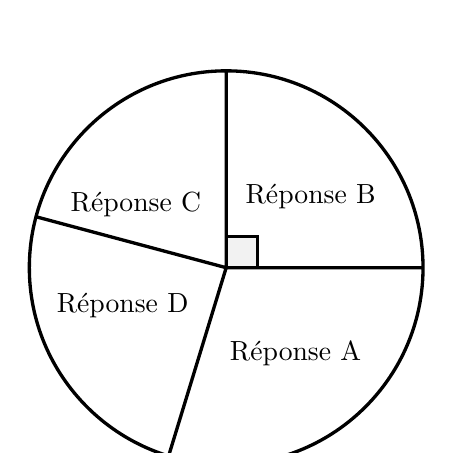
\begin{tikzpicture}[baseline={(0,0)}]
	\draw[line width=1pt, fill=gray!10] (0,0) rectangle (0.4,0.4) ;
	\draw[line width=1.2pt] (0,0)circle (2.5)
		(0,0)--(0:2.5)
		(0,0)--(-107:2.5)
		(0,0)--(90:2.5)
		(0,0)--(165:2.5);
	\node at (-51:1.4) {Réponse A};
	\node at (40:1.4) {Réponse B};
	\node at (145:1.4) {Réponse C};
	\node at (200:1.4) {Réponse D};
\end{tikzpicture}
\hfill~

%%%% pstricks
%\begin{flushright}
%\psset{unit=0.9cm,linewidth=1.5pt}
%\def\xmin{-3}   \def\xmax{3} \def\ymin{-3}   \def\ymax{3}
%\begin{pspicture}(\xmin,\ymin)(\xmax,\ymax)
%\psline(0,3)(0,0)(3,0) \psframe[fillstyle=solid,fillcolor=lightgray](0,0)(0.4,0.4)
%\psline(3;160)(0,0)(3;250)
%\pscircle(0,0){3}
%\rput(1.4,1){Réponse B} \rput(1.3,-1.2){Réponse A} 
%\rput(-1.4,1.3){Réponse C} \rput(-1.5,-0.5){Réponse D} 
%\end{pspicture}
%\end{flushright}

\subsection*{Question 8}
\begin{minipage}{0.5\linewidth}
	Parmi les propositions suivantes, laquelle est le périmètre de la figure ci-contre?

\medskip
\begin{tblr}{colspec = {*2{X[c]}}}
	\textbf{A.}\quad \np[mm]{30}   &
	\textbf{B.}\quad \np[mm^2]{30} \\
 	\textbf{C.}\quad \np[mm]{50}   &
 	\textbf{D.}\quad \np[mm^2]{50} \\
 \end{tblr}
\end{minipage}
 \hfill~
 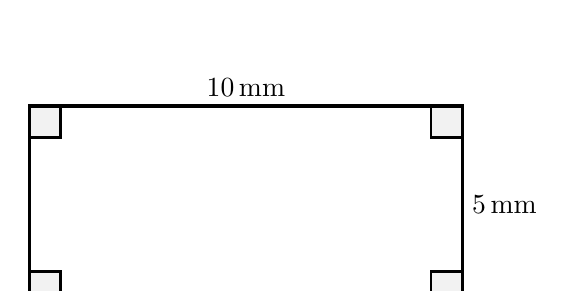
\begin{tikzpicture}[baseline={(0,1.25)}]
 	\draw[line width=1pt, fill=gray!10] (0,0) rectangle ++(0.4,0.4) ;
 	\draw[line width=1pt, fill=gray!10] (0,2.1) rectangle ++(0.4,0.4) ;
 	\draw[line width=1pt, fill=gray!10] (5.1,0) rectangle ++(0.4,0.4) ;
 	\draw[line width=1pt, fill=gray!10] (5.1,2.1) rectangle ++(0.4,0.4) ;
 	\draw[line width=1.2pt] (0,0) rectangle (5.5,2.5);
 	\node[above] at (2.75,2.5) {\np[mm]{10}};
 	\node[right] at (5.5,1.25) {\np[mm]{5}};
 \end{tikzpicture}
 \hfill~

%%%% pstricks
%\begin{flushright}
%\psset{unit=0.5cm,linewidth=1.5pt}
%\def\xmin {0}   \def\xmax {12} \def\ymin{0}   \def\ymax{6}
%\begin{pspicture}(\xmin,\ymin)(\xmax,\ymax)
%\psframe(0,0)(10,5)
%\psset{fillstyle=solid,fillcolor=lightgray}
%\psframe(0,0)(0.5,0.5) \psframe(0,5)(0.5,4.5)
%\psframe(10,0)(9.5,0.5) \psframe(10,5)(9.5,4.5) 
%\uput[u](5,5){$10$ mm} \uput[r](10,2.5){$5$ mm}
%\end{pspicture}
%\end{flushright}

\subsection*{Question 9}
Parmi les propositions suivantes, laquelle donne le cosinus de l'angle $\widehat{\mathrm{EDF}}$ dans le triangle rectangle ci-dessous ?

\medskip
\begin{tblr}{colspec = {*4{X[c]}}}
	\textbf{A.}\quad $\dfrac{4}{5}$&
	\textbf{B.}\quad $\dfrac{3}{5}$&
	\textbf{C.}\quad $\dfrac{5}{3}$&
	\textbf{D.}\quad $\dfrac{4}{3}$\\
\end{tblr}

\begin{center}
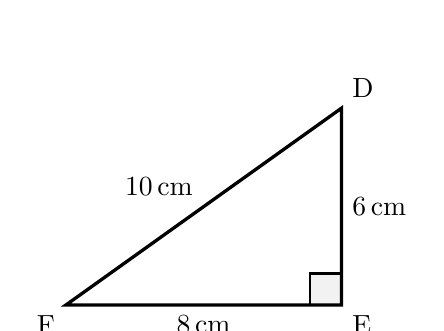
\begin{tikzpicture}[baseline={(0,1.25)}]
	\draw[line width=1pt, fill=gray!10] (3.1,0) rectangle ++(0.4,0.4) ;
	\draw[line width=1.2pt] (0,0)node[below left]{F}
	-- (3.5,2.5)node[above right]{D} node[pos=0.5,above left]{\np[cm]{10}}
	-- (3.5,0)node[below right]{E} node[pos=0.5,right]{\np[cm]{6}}
	-- cycle node[pos=0.5,below]{\np[cm]{8}};
\end{tikzpicture}
\end{center}

%%%% pstricks
%\begin{center}
%\psset{unit=0.5cm,linewidth=1.5pt}
%\def\xmin {-9}   \def\xmax {2} \def\ymin{-1}   \def\ymax{7}
%\begin{pspicture*}(\xmin,\ymin)(\xmax,\ymax)
%\pspolygon(-8,0)(0,0)(0,6)
%\psframe[fillstyle=solid,fillcolor=lightgray](-0.5,0.5)(0,0)
%\uput[ur](0,6){D} \uput[dr](0,0){E} \uput[dl](-8,0){F}
%\uput[d](-4,0){$8$ cm} \uput[r](0,3){$6$ cm}
%\uput[ul](-4,3){$10$ cm}
%\end{pspicture*}
%\end{center}

\needspace{25\baselineskip}
\section*{\centering DEUXIÈME PARTIE (14 points)}

\needspace{10\baselineskip}
% saut de page si moins de 10 lignes disponibles
\section*{Exercice 1 (3 points)}
Le tableau ci-dessous présente le nombre de médailles obtenues par 9 pays lors des Jeux Paralympiques de Paris 2024.

\begin{center}
	\begin{tblr}{hlines, vlines, colspec={X[l,4cm]*{4}{X[c,2cm]}}}
		Pays            & Or & Argent & Bronze & Total \\
		Chine           & 94 & 76     & 50     & 220   \\
		Grande-Bretagne & 49 & 44     & 31     & 124   \\
		États-Unis      & 36 & 42     & 27     & 105   \\
		Pays-Bas        & 27 & 17     & 12     & 56    \\
		Brésil          & 25 & 26     & 38     & 89    \\
		Italie          & 24 & 15     & 32     & 71    \\
		Ukraine         & 22 & 28     & 32     & 82    \\
		France          & 19 & 28     & 28     & 75    \\
		Australie       & ?  & 17     & 28     & 63
	\end{tblr}
\end{center}

\begin{enumerate}
	\item Combien de médailles d'or ont été obtenues par les Pays-Bas?

	\item Calculer le nombre de médailles d'or obtenues par l'Australie.

	\item Montrer que l'affirmation suivante est vraie.

	« Plus de $20~\%$ des médailles obtenues par la Grande-Bretagne sont en bronze.»

	\item \begin{enumerate}
		\item Déterminer la médiane de la série des nombres de médailles obtenues par ces 9 pays (colonne « Total » du tableau).

		\textbf{Détailler la réponse en précisant la démarche.}

		\item Interpréter ce résultat dans le contexte de l'exercice.
	\end{enumerate}

	\item Aux Jeux Paralympiques de Tokyo en 2021, le Brésil avait obtenu 20 médailles d'argent. Pour ceux de Paris en 2024, il a obtenu 26 médailles d'argent.

	Quel est le pourcentage d'augmentation du nombre de médailles d'argent obtenues par le Brésil entre 2021 et 2024 ?
\end{enumerate}

\needspace{10\baselineskip}
% saut de page si moins de 10 lignes disponibles
\section*{Exercice 2 (4 points)}
	Sur la figure ci-dessous :

\begin{itemize}[left=5mm]
	\item les droites (BD) et (CE) sont sécantes en A;
	\item les droites (BC) et (DE) sont parallèles;
	\item $\mathrm{AB}=\np[cm]{6,4}$;\quad
	$\mathrm{AC}= \np[cm]{4,8}$;\quad
	$\mathrm{AD}= \np[cm]{4,8}$;\quad
	$\mathrm{BC}= \np[cm]{8}$.
\end{itemize}
\begin{center}
	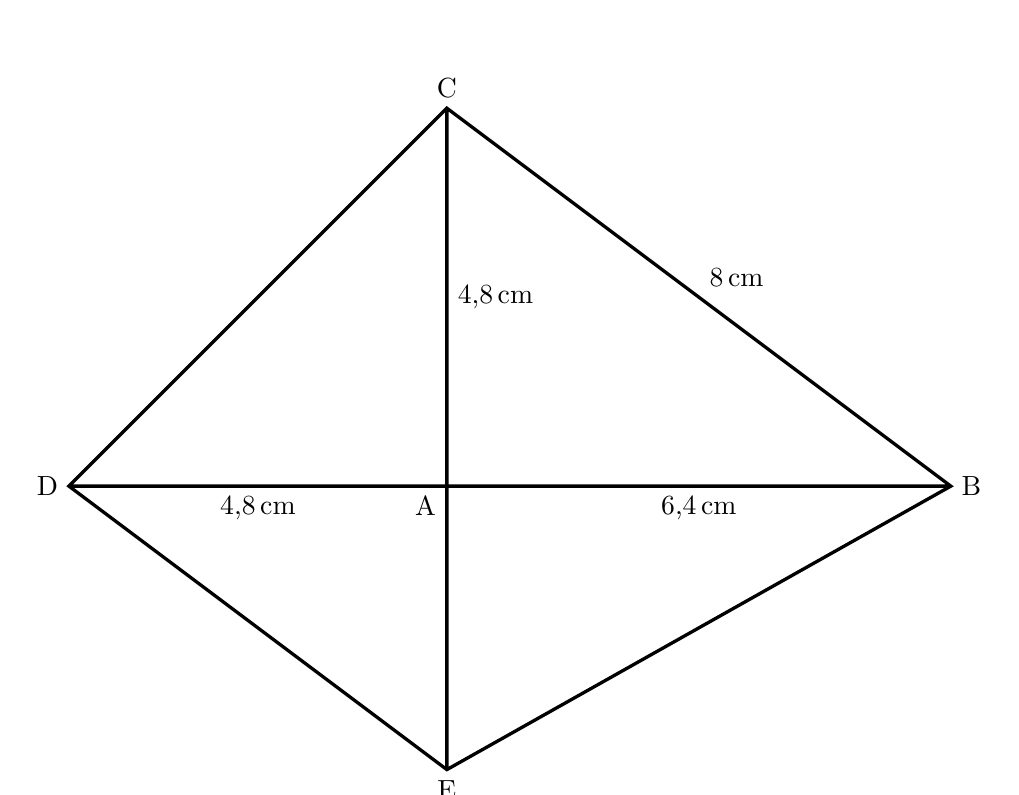
\begin{tikzpicture}[baseline={(0,1.25)}]
		\draw[line width=1.2pt] (0,0)node[below left]{A}
		(6.4,0)node[right]{B}
		-- (0,4.8)node[above]{C} node[pos=0.5,above right]{\np[cm]{8}}
		-- (-4.8,0)node[left]{D}
		-- (0,-3.6)node[below]{E}--cycle
		(6.4,0)--(0,0) node[pos=0.5,below]{\np[cm]{6,4}}
		(-4.8,0)--(0,0) node[pos=0.5,below]{\np[cm]{4,8}}
		(0,4.8)--(0,0) node[pos=0.5,right]{\np[cm]{4,8}}
		(0,-3.6)--(0,0);
	\end{tikzpicture}
\end{center}

%%%% pstricks
%\begin{center}
%\psset{unit=1cm,linewidth=1.5pt}
%\def\xmin {-6}   \def\xmax {7} \def\ymin{-5}   \def\ymax{6}
%\begin{pspicture*}(\xmin,\ymin)(\xmax,\ymax)
%\pspolygon(-4.8,0)(0,4.8)(6.4,0)(0,-3.6)
%\psline(-4.8,0)(6.4,0) \psline(0,4.8)(0,-3.6)
%\uput[d](-2.4,0){$4,8$ cm} \uput[d](3.2,0){$6,4$ cm}
%\uput[r](0,2.4){$4,8$ cm} \uput[ur](3.2,2.4){$8$ cm}
%\uput[dl](0,0){A} \uput[r](6.4,0){B} \uput[u](0,4.8){C}
%\uput[l](-4.8,0){D}  \uput[d](0,-3.6){E}   
%\end{pspicture*}
%\end{center}

\begin{enumerate}
	\item Montrer que le triangle ABC est rectangle en A.

	\item Montrer que $\mathrm{DE}=\np[cm]{6}$ et $\mathrm{AE}= \np[cm]{3,6}$.

	\item Montrer que les angles $\widehat{\mathrm{ABC}}$ et $\widehat{\mathrm{ADE}}$ sont égaux.

	\textbf{Détailler la réponse en précisant la démarche.}

	\item Montrer que les triangles ABC et ADE sont semblables.

	\item Déterminer l'aire du quadrilatère BCDE.
\end{enumerate}


\needspace{10\baselineskip}
% saut de page si moins de 10 lignes disponibles
\section*{Exercice 3 (3 points)}
\textbf{Dans cet exercice, les parties A et B sont indépendantes.}

\medskip

\begin{minipage}[t]{0.47\linewidth}
\subsection*{Partie A}
On a tracé ci-contre la courbe représentative de la fonction qui donne le volume d'une boule en~$\mathrm{cm}^{3}$ en fonction de son rayon en~cm.

\begin{enumerate}
	\item Déterminer graphiquement l'image de 3,6 par cette fonction.

	\item Le volume d'une boule est égal à \np[cm^3]{660}.

	Lire graphiquement son rayon.
\end{enumerate}
\end{minipage}
\hfill~
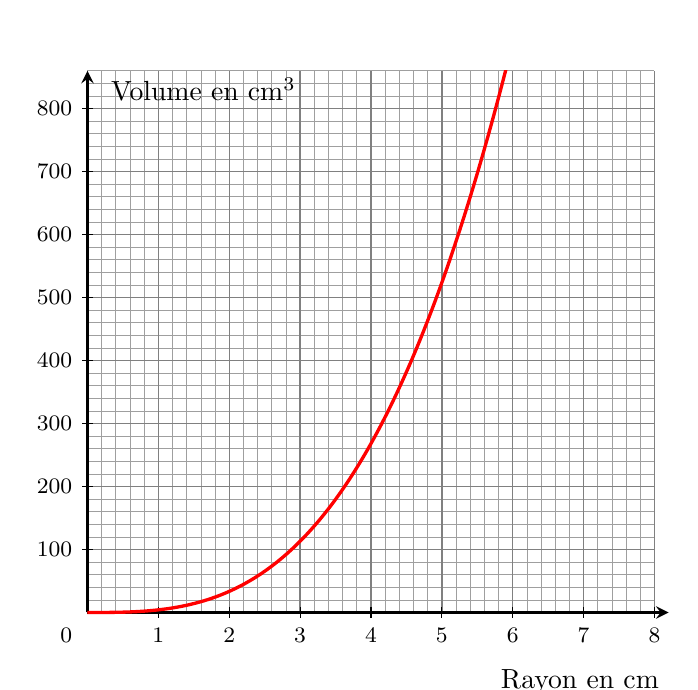
\begin{tikzpicture}[x=9mm,y=0.08mm,baseline={(vol.base)},> =stealth]
	\draw [color = gray!75, line width = 0.25pt, xstep=0.2, ystep = 20] (0,0) grid (8,860);
	\draw [color = gray, line width = 0.5pt, xstep=1, ystep = 100] (0,0) grid (8,860);
	\draw[->,line width=1pt] (0,0) -- (8.2,0);
	\node[left] at (8.2,-25pt) {Rayon en cm};
	\foreach \x in {1,...,8}
	\draw[shift={(\x,0)},color=black] (0pt,2pt) -- (0pt,-2pt) node[below, fill = white] {\footnotesize $\np{\x}$};
	\draw[->,line width=1pt] (0,0) -- (0,860);
	\node[right] (vol) at (5pt,830) {Volume en $\mathrm{cm}^3$};
	\foreach \y in {100,200,...,800}
	\draw[shift={(0,\y)},color=black] (2pt,0pt) -- (-2pt,0pt) node[left, fill = white] {\footnotesize $\np{\y}$};
	\draw[color=black] (-2pt,-2pt) node[below left] {{\footnotesize 0}};
	\clip (0,-2pt) rectangle (8,860);
	\draw[line width=1.2pt,color=red,smooth,samples=100,domain= 0:6] plot(\x,{4.18879*\x*\x*\x});
\end{tikzpicture}
\hfill~


%%%% pstricks
%\begin{flushright}
%\psset{xunit=1cm,yunit=0.01cm,linewidth=1.5pt,arrowsize=2pt 3,comma}
%\def\xmin{-1}   \def\xmax{8.4} \def\ymin{-100}   \def\ymax{880}
%\begin{pspicture*}(\xmin,\ymin)(\xmax,\ymax)
%\psgrid[yunit=1cm,subgriddiv=5,  gridlabels=0, subgridcolor=lightgray!50,gridcolor=lightgray](0,0)(\xmax,9)
%\psaxes[labelFontSize=\footnotesize,Dy=100, ticksize=-2pt 2pt,]{->}(0,0)(0,0)(\xmax,\ymax)
%\psplot[linecolor=blue,plotpoints=3000]{0}{\xmax}{4 3.14159 mul x 3 exp mul 3 div}
%\uput[r](0.4,840){Volume en cm$^3$}
%\uput[d](7,-40){Rayon en cm}
%\end{pspicture*}
%\end{flushright}

\subsection*{Partie B}
On souhaite fabriquer avec une imprimante 3D, des boules pleines en plastique, de rayon de \np[cm]{2,5}.

\begin{enumerate}
	\item Montrer que le volume d'une boule, arrondi à l'unité, est égal à \np[cm^3]{65}.

	\emph{On rappelle que le volume $V$ d'une boule de rayon $R$ est donné par la formule :}

	$V=\dfrac{4}{3} \times \pi \times R^{3}$

	\item Pour utiliser cette imprimante, on dispose d'une bobine de \np[cm^3]{1000} de plastique.

	Combien de boules peut-on fabriquer au maximum ?

	\item Sachant que la masse volumique de ce plastique est égale à \np[g/cm^3]{0,9}, calculer la masse d'une boule.
\end{enumerate}

\needspace{10\baselineskip}
% saut de page si moins de 10 lignes disponibles
\section*{Exercice 4 (2 points)}
On souhaite réaliser des sachets de bonbons.

Pour cela, on dispose de 112 bonbons à la fraise et de 140 bonbons au caramel.

\begin{itemize}[left=5mm]
	\item Tous les sachets contiennent le même nombre de bonbons à la fraise.

	\item Tous les sachets contiennent le même nombre de bonbons au caramel.

	\item Tous les bonbons à la fraise et au caramel sont utilisés.
\end{itemize}

\begin{enumerate}
	\item Peut-on constituer 16 sachets?

	\item La décomposition en facteurs premiers de 112 est $2^{4} \times 7$.

	Quelle est la décomposition en facteurs premiers de 140 ?

	\item Quel nombre maximal de sachets pourra-t-on constituer ?

	Quelle sera alors la composition de chaque sachet?
\end{enumerate}

% Fin du document
\end{document}